\chapter{Object Reconstruction}
\label{sec:object_reconstruction}

This chapter will overview the methods used to reconstruct the objects in each event, that are critical for the searches described in Chapters~\ref{sec:bsm_H_to_tau_tau_analysis} and~\ref{sec:H_A_to_4_tau_analysis}.
The topics discussed here are the reconstruction of tracks and vertices, the particle flow algorithm, the calculation of the \ac{MET}, the measurements of jets and the tagging of their flavours, and the identification of electrons, muons, and tau leptons.

\section{Tracks and vertices}

The \ac{CTF} algorithm~\cite{CMS:2014pgm} is employed by \ac{CMS} to reconstruct particle tracks. 
This algorithm consists of four steps to estimate trajectory parameters and uncertainties. 
Initially, track seeds are formed using hits in the first few layers of the tracker. 
These seeds provide initial estimates of the trajectory. 
Next, the track seeds are extrapolated using a Kalman filter~\cite{Fruhwirth:1987fm}, searching for additional hits along the expected trajectory in successive detector layers. 
The trajectory parameters are continuously updated as hits are added to the track candidate. 
The extrapolation process continues until the final detector layer is reached. \\

Afterwards, a Kalman filter and smoother are used to fit the final trajectory iteratively. 
Spurious hits are identified and removed after each iteration until no more spurious hits are found. 
This fitting process provides the most accurate estimates of the trajectory parameters. 
Subsequently, tracks must pass a set of quality criteria, and any failing tracks are discarded. \\

The \ac{CTF} algorithm performs six iterations, gradually reconstructing more challenging tracks and recovering missed tracks from previous iterations. 
Associated hits are removed after each iteration, reducing combinatorial complexity and facilitating the search for complicated tracks in later iterations. 
Tracking efficiencies for muons and pions with transverse momentum ($\pT$) greater than 500 MeV have been measured to be over 99.3\% and 98.5\%, respectively~\cite{CMS:2010mua}. \\

Once all tracks are reconstructed, the positions of interaction vertices, including the primary vertex and additional vertices from \ac{PU}, are determined. 
Vertex reconstruction begins by selecting tracks consistent with being promptly produced near the beamspot. 
Tracks are then clustered based on the z coordinate of their closest approach to the beamspot, using a deterministic annealing algorithm~\cite{Rose:1998dzq}. 
Candidate vertices are retained if at least two of their associated tracks are incompatible with other vertices. 
The candidate vertices are fitted using an adaptive vertex fitter~\cite{Fruhwirth:2007hz} to determine the best estimate of their three dimensional positions. 
The primary interaction vertex is determined as the vertex with the highest summed physics-object $\pT$, where physics objects are jets clustered from tracks associated with the candidate vertex using the anti-$k_T$ algorithm~\cite{Fruhwirth:2007hz}.
The efficiency of vertex reconstruction has been measured, with values exceeding 98.7\% for vertices containing at least two tracks and exceeding 99.9\% for vertices with four or more tracks~\cite{CMS:2010mua}. 

\section{Particle flow}

The \ac{PF} algorithm~\cite{PF_CMS,CMS:2010byl,CMS:2010eua} is used for the reconstruction of stable particles in an event, such as electrons, photons, muons, and hadrons. 
This algorithm combines information from all the sub-detectors of \ac{CMS} to achieve accurate measurements of particle energies, directions, and types. 
The output of the algorithm is a list of particles, which can then be used to construct higher-level objects like jets, hadronically decaying taus, and the \ac{MET}.\\

The \ac{PF} algorithm begins with information about the tracking and calorimeter clustering.
The tracking information includes the high resolution momentum and direction of charged hadrons calculated by an iterative-tracking strategy~\ref{Adam:934067}, that is not achievable with the calorimeters.
The calorimeter clustering is crucial for measuring the energies and directions of neutral particles, distinguishing energy deposits from neutral and charged hadrons, and identifying bremsstrahlung photons originating from electrons.
Clusters are 
Clustering is performed separately in each sub-detector component except for the \ac{HF} sub-detector. \\

Clustering starts with \say{cluster seeds} consisting of cells with local energy maxima above a certain threshold. 
Neighbouring cells are aggregated into \say{topological clusters} if their energies are above the expected noise levels. 
Each topological cluster gives rise to one or more \say{particle flow clusters}. 
The energy of each cell can be shared among multiple particle flow clusters based on the cell-cluster distance. \\

To establish links between elements, a distance parameter is defined to quantify the quality of the link. 
Tracks are extrapolated to different detector layers, and if the extrapolated position is within the cluster boundaries, a link is made between the track and the cluster. 
Tangents to the tracks are also extrapolated to the \ac{ECAL}, and if within a cluster, they are linked as potential bremsstrahlung photons. 
Links between calorimeter clusters are established if the position of the more granular cluster is within the boundaries of the less granular calorimeter. 
The linking distance parameter is defined as the distance between the extrapolated position and the cluster center. \\

The \ac{PF} algorithm then combines directly or indirectly linked elements into blocks, typically containing 1-3 elements. 
From each block, particles are identified through a series of tests. 
A global muon is identified if a track is linked to a muon system track and their momenta are compatible. 
\ac{PF} electrons are identified by refitting candidate tracks using a \ac{GSF} and evaluating their compatibility with \ac{ECAL} clusters using multivariate discriminants. 
Remaining tracks lead to \ac{PF} charged hadrons, and their momenta are determined by track fits, with adjustments made by matching the calorimetric energy. 
Excess energy not consistent with track momenta is attributed to overlapping photons and neutral hadrons. \\

Lastly, any remaining \ac{ECAL} and \ac{HCAL} deposits are used to identify \ac{PF} photons and \ac{PF} neutral hadrons, respectively. 
This comprehensive process of reconstruction and identification ensures precise measurements of stable particles within the \ac{CMS} detector.

\section{Muons}

Muons are required to be reconstructed as muon by the particle flow reconstruction. They additionally must pass \textit{Medium muon} requirements~\cite{cmsMediumMuon}, 
as recommended by the Muon POG. These requirements are:
\begin{itemize}
\item The muon is reconstructed by the \textit{tracker} or \textit{global} muon reconstruction algorithm.
\item The impact parameters $d_{xy}$ and $d_{z}$ between the muon track ('best track') 
and the primary vertex are restricted as $d_{xy}<0.045$~cm and $d_{z}<0.2$~cm to ensure the muon is associated with the primary vertex
\item At least 80\% of the tracker hits have to be valid
\end{itemize}
In addition, either of the following two sets of criteria must be satisfied:
\begin{itemize}
\item The muon is reconstructed by the \textit{global} muon reconstruction algorithm.
\item The $\chi^2$/ndof of the global track fit is smaller than 3
\item The $\chi^2$ of the tracker-standalone position match is smaller than 12
\item The $\chi^2$ of the track kink finder is less than 20
\item The muon segment compatibility is $>$ 0.303
\end{itemize}
\textit{or}:
\begin{itemize}
\item The muon segment compatibility is $>$ 0.451 
\end{itemize}

\textbf{Isolation}~\\
To reduce the contamination from muons originating from heavy-flavoured quark decays in jets or decays in flight, selected muons are required to be isolated. The isolation is based on photon and neutral/charged hadron particle flow candidates within a cone size of $\Delta R<0.4$ of the selected muon. A relative combined isolation variable is defined as:

\begin{equation}
\label{eqn:reliso}
I_{rel}^{\mu} = \frac{\Sigma P_{T}(\text{charged}) + \mathrm{max}(\Sigma E_{T}(\text{neutral}) + \Sigma E_{\text{T}}(\text{photon}) - \Delta\beta \Sigma E_{\text{T}}(\text{PU}),0)}{P_{\text{T}}^{\mu}},
\end{equation}

where $P_{T}(\text{charged})$ corresponds to the $P_{T}$ of all charged hadronic candidates from primary vertex, $E_{T}(\text{photon, neutral})$ 
to the transverse energy of all photon and neutral hadron candidates, and $\Delta \beta$ is the energy estimate of neutral particles due to pileup, which is taken to be 0.5.
Furthermore $E_{\text{T}}(\text{PU})$ corresponds to the transverse momentum of all charged hadronic candidates from pileup.
The muon isolation used is $I_{rel}<0.15$.

\begin{figure}[!hbtp]
\centering
    \subfloat[]{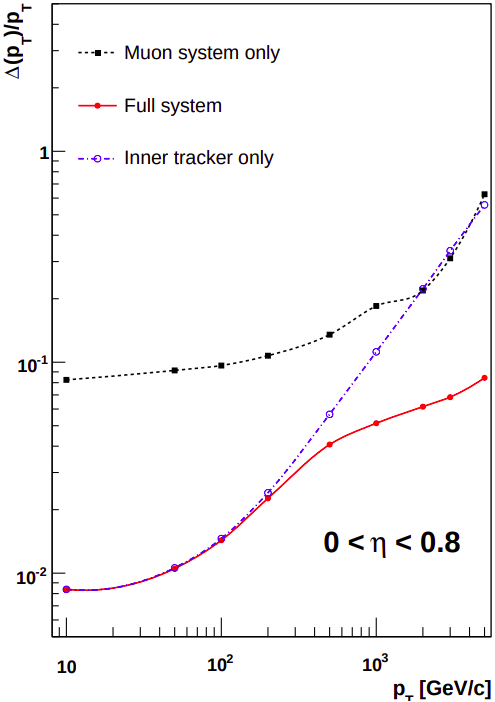
\includegraphics[width=0.5\textwidth]{Figures/muon_res_loweta.png}}
    \subfloat[]{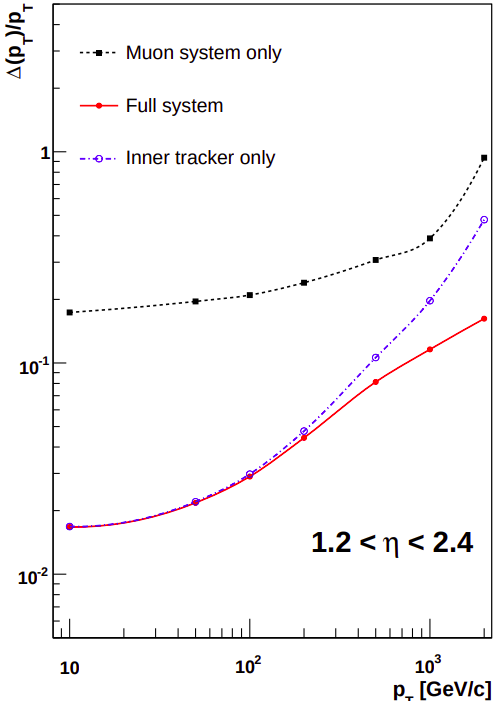
\includegraphics[width=0.5\textwidth]{Figures/muon_res_higheta.png}} \\
\caption{The $\pT$ resolution for muon identification using the muon system (black), the inner tracker (blue), and the full system (red). This is shown for the pseduorapidity regions $0 < \eta < 0.8$ (a) and  $1.2 < \eta < 2.4$ (b)}
\label{fig:muon_eff}
\end{figure}

\section{Electrons}

In addition, electrons are required to pass an identification variable based on a \ac{BDT} discriminator which uses track quality, shower shapes and kinematic quantities as input.
The following variables are used as input to the BDT:  ~\cite{cmsElectron}
\begin{itemize}
\item Cluster shape variables $\sigma_{i\eta,i\eta}$ and $\sigma_{i\phi,i\phi}$, with $i\eta$ and $i\phi$ the integer
label of the $\eta$ and $\phi$ calorimeter cell. The circularity =  $1 -\frac{E1\times5}{E5\times5}$, with
$E1\times5$ and $E5\times5$ the energies in a $1\times5$ and a $5\times5$ grid around the super cluster seed,
respectively. Shape variable R9 = $\frac{E3\times3}{E_{SC}}$, with $E3\times3$ the energy in a $3\times3$ grid
of cells around the super cluster seed and $E_{SC}$ the raw energy of the super cluster.
\item The number of valid hits in the track fit, the $\chi^2$ of the track fit and the $\chi^2$ of the GSFTrack fit
\item The number of GSFtrack hits, the number of expected missing inner hits and the result of the conversion vertex fit
\item The distance $\Delta \eta$ and $\Delta \phi$ between the reconstructed super cluster and the associated track at the position of the primary vertex, and the distance in $\eta$ between the super cluster and the track at the calorimeter surface.
\item H/E, the ratio of the hadronic energy over the electromagnetic energy in the super cluster and E/P, the ratio of the super cluster energy over the momentum of the track associated with the electron 
\item The ratio of the energy of the electron cluster and the momentum of the associated track, evaluated at the electron cluster,
 and $1/E_e - 1/P_e$, with $E_e$ the energy of the electron candidate and $P_e$ its momentum.
\end{itemize}
The BDT was trained on a $Z/\gamma^{*}$ Monte Carlo sample generated with
\texttt{MadGraph 5}, in 3 $\eta$ bins for electrons with $p_{\text{T}}>10$ GeV.
This analysis uses the version of the ID BDT without the isolation included in
the training, instead using an additional cut on the electron isolation. This
was shown to give similar performance to the version of the ID including the
isolation and makes defining side-band regions used for estimation of
backgrounds simpler.

The electron are additionally required to pass the 90\% efficiency working point. Finally electrons are also subject to the same impact parameter requirements as the
muons: the impact parameters $d_{xy}$ and $d_{z}$ between the electron track 
and the primary vertex are restricted as $d_{xy}<0.045$~cm and $d_{z}<0.2$~cm to
ensure the electron is associated with the primary vertex.

The isolation used is based on photon and neutral/charged hadron particle flow
candidates within a cone size of $\Delta R<0.3$ of the selected electron but
used a different method to estimate the neutral particles due to pileup, namely
the rho--effective-area method. The pileup in this method is estimated as
$PU=\rho\cdot\text{EA}$, where $\rho$ is the event-specific average pile-up
energy density per unit area in the $\phi$-$\eta$ plane and the EA is the
effective area specific to the given type of isolation. The rho--effective-area
subtracted relative combined isolation variable is defined as:
\begin{equation}
\label{eqn:electron_reliso_rho} 
I_{\text{rel}}^{e} = \frac{\Sigma
    P_{T}(\text{charged}) + \mathrm{max}(\Sigma E_{T}(\text{neutral}) + \Sigma
E_{T}(\text{photon}) - \rho\cdot\text{EA},0)}{P_{T}^{e}}, \end{equation} where
the $\text{EA}$ is measured in bins of $\eta$ as listed in Table
\ref{tab:EleEA}. The electron isolation used is $I_{rel}<0.15$. 

\begin{table}[htb]
\begin{center}
{\footnotesize
\begin{tabular}{|c|c|}
\hline
$\eta$ range & EA \\
\hline
0.0$\leq\eta<$1.0   &  0.1440 \\
1.0$\leq\eta<$1.479 &  0.1562 \\
1.479$\leq\eta<$2.0 &  0.1032 \\
2.0$\leq\eta<$2.2   &  0.0859 \\
2.2$\leq\eta<$2.3   &  0.1116 \\
2.3$\leq\eta<$2.4   &  0.1321 \\
2.4$\leq\eta<$5.0   &  0.1654 \\
\hline
\end{tabular}
} % end footnotesize
\end{center}
\caption{
 Electron effective areas used for the $\rho$-corrected isolation computation.
}
\label{tab:EleEA}
\end{table}

\section{Jets}

Jets are clustered from all particle flow  candidates using the anti $k_{\text{T}}$ algorithm~\cite{Cacciari:2011ma} with a cone size parameter R=0.4. 
To reduce the contribution of jets that originate from pile--up vertices, charged hadrons that are not associated with the hard--scattering primary vertex are removed from the particle flow candidates 
that form the input to the anti-$k_{\text{T}}$-algorithm (charged hadron subtraction).

The jets are required to pass the tight working point of
the PF jet ID discriminator provided by the jetMET POG~\cite{PFJetID}.  
To exclude selected $e,\mu,\tau_{h}$ candidates from the jet collection, the jets
are required to be separated from the selected $\tau$ candidate by $\Delta R
> 0.5$.  Jets with a corrected $p_{\text{T}} > 30$ GeV and $|\eta|<4.7$ are
considered.

High endcap ECAL noise in 2017 led to large amounts of noise in reconstructed jets~\cite{JetTwiki}. To mitigate the noise issue,
jets reconstructed on 2017 data also used a veto of jets with
raw $p_{t} < 50$ and $2.65 < |\eta| < 3.139$. 

\section{b jets}

For determining whether a jet is initiated by a b quark, the \texttt{DeepJet} algorithm~\cite{CMS:2017wtu,Bols:2020bkb} is used.  
This heavy-flavour jet identifier, uses properties of the jet to distinguish jets originating from b quarks, c quarks, the remainder of the lighter quarks grouped, and gluons.
Core to the b tagging in this algorithm is the reconstruction of a \ac{SV} due to the lifetime of b quarks, allowing for displaced tracks.
The \texttt{DeepJet} \ac{DNN} uses a combination of high-level variables such as the \ac{SV}, as well as utilising low-level variable of jet constituents to separate between initiators.
The \ac{DNN} uses a mixture of convolutional and dense layers to perform this categorisation. \\

For b jet selection, jets are required to have $\pT > 20$ GeV and $|\eta| <$ 2.4 (2.5) in 2016 (2017 and 2018), and are considered b tagged if their discriminator value is larger than some threshold that represents a mis-identification rate of 1\%.
This corresponds to a b tagging efficiency around 80\%.

\begin{figure}[!hbtp]
\centering
    \subfloat[]{\includegraphics[width=0.8\textwidth]{Figures/deepjet.pdf}}
\caption{Mis-identification probability 2$\sigma$ bands against efficiency for b tagging using the \texttt{DeepJet} algorithm, for AK4jets with $\pT> 30$ GeV AND $|\eta|$<2.5 utilising MC with parameters from the 2017 era of data taking. Two bands are displayed, one for the identification of a b quark rather than light quarks and gluons (blue) and one for the identification of a b quark rather than a c quark (red)~\cite{deepjet}.}
\label{fig:deeptau_misid}
\end{figure}

\section{Missing transverse energy}

The \ac{MET} is used as a feature to understand particles passing through the \ac{CMS}, such as neutrinos in the \ac{SM}, and weakly interacting particles from hypothetical \ac{BSM} extensions.
This information cannot be pulled from the detector itself but instead the absence of detection can be used to infer the presence of such an object
The \ac{MET} is nominally calculated as the negative vector sum of all transverse momenta of the \ac{PF} candidates in the collision event,

\begin{equation}
\vec{E}_{T}^{\text{miss}} = - \sum_{i} \vec{p}_{T}^{\hspace{4pt}i}.
\end{equation}

However, this raw \ac{PF}\ac{MET} is inaccurate due to the $\pT$ thresholds of the calorimeters, the non-linearity of the calorimeter response and due to reconstruction inefficiencies~\cite{CMS:2016ljj}.
This is fixed with jet energy corrections, determined for jets with $\pT$> 15 GeV and less than 90\% for their energies deposited in the \ac{ECAL} for each of the problems mentioned, and then the corrected \ac{MET} is calculated by,

\begin{equation}
\vec{E}_{T}^{\text{miss,corr}} = \vec{E}_{T}^{\text{miss}} - \sum_{\text{jets}} (\vec{p}_{T,\text{jet}}^{\text{\hspace{4pt}corr}} - \vec{p}_{T,\text{jet}}^{\text{\hspace{4pt}raw}}),
\end{equation}

where \say{corr} and \say{raw} are the corrected and uncorrected values of the jet momenta, respectively. \\

Further corrections are required to account for \ac{PU} effects, and the \texttt{PUPPI} algorithm is used for this purpose~\cite{CMS:2020ebo}.
The algorithm is designed to address the impact of \ac{PU} on observables involving clustered hadrons, such as jets, missing transverse momentum, and lepton isolation. 
It achieves this by combining information about the local particle distribution, event \ac{PU} properties, and tracking data. 
\texttt{PUPPI} operates at the level of individual particle candidates, before any clustering is performed. 
It assigns a weight to each particle, ranging from 0 to 1, based on the information from surrounding particles. 
A weight of 1 is given to particles believed to originate from the \ac{PV}. 
These per-particle weights are then used to rescale the four-momenta of the particles, effectively correcting for the impact of \ac{PU} and so altering the raw calculation of the \ac{MET} to,

\begin{equation}
\vec{E}_{T}^{\text{miss}} = - \sum_{i} w_{i} \cdot \vec{p}_{T}^{\hspace{4pt}i}.
\end{equation}

\section{Taus}

Fundamental to this thesis is the identification of tau particles.
The tau lepton is measured to have a mean lifetime of \(2.9 \times 10^{-13}\)s. 
This short lifetimes means that the tau lepton is not directly observable in the \ac{CMS} detector.  
In order to detect these particles, it is important to understand how the tau decays. 
Due to the heavy nature of the particle, it does not only decay leptonically, but unlike the muon, it can also decay hadronically.
A list of prominent decays of the tau lepton are shown in the Table~\ref{tab:tau_decay}.
These decays can be split into three groups: the 17.8\% of taus that decay to an electron ($e$), the 17.4\% that decay into a muon ($\mu$), and hadronic tau decays ($\tauh$) that make up the final 64.8\% of tau decays. 
The leptonic decays of the tau can be accounted for by the identification of electrons and muons as discussed in the previous subsection.  \\

\begin{table}[h]
    \centering
    \begin{tabular}{|c|c|}
         \hline
         Decay Mode & Branching Fraction  \\
         \hline
         \hline
         \textbf{Leptonic Decay ($e$, $\mu$)} & \textbf{35.2\%} \\
         $e^- \bar{\nu}_e \nu_\tau $ & 17.8\% \\
         $\mu^- \bar{\nu}_\mu \nu_\tau $ & 17.4\% \\
         \hline
         \textbf{Hadronic Decay ($\tauh$)} & \textbf{64.8\%} \\
         $h^- \pi^0 \nu_\tau $ & 25.9\% \\
         $h^- \nu_\tau$ & 11.5\% \\
         $h^- h^+ h^+ \nu_\tau$ & 9.8\% \\
         $h^- 2\pi^0 \nu_\tau$ & 9.3\% \\
         $h^- h^+ h^- \pi^0 \nu_\tau$ & 4.8\% \\
         other & 3.2\% \\
         \hline
    \end{tabular}
    \caption{Measured branching fractions for the tau lepton. h represents a charged hadron either a pion or a kaon~\cite{ParticleDataGroup:2022pth}.}
    \label{tab:tau_decay}
\end{table}

A two step process is used to identify hadronic taus.
The \ac{HPS} algorithm is used to initially identify hadronic taus based on jets produced by the anti-$k_{\text{T}}$ algorithm with a distance parameter of $\Delta R = 0.4$. 
To capture the energy deposits left by $\pi^0$ candidates in the ECAL, the photon and electron constituents of the jet responsible for seeding the tau reconstruction are assembled into strips. 
All electrons or photons used are required to have $p_{\text{T}} > 0.5$ GeV.
The initial iteration of the \ac{HPS} algorithm used a fixed strip size of $\Delta \eta \times \Delta \phi$ equal to $0.05 \times 0.20$.
However, this technique was updated to a dynamical strip size to account for the multiple scatterings of $e^+ e^-$ products from a $pi^0$ decay, falling outside of the fixed window.
A reliance of the hadronic tau $\pT$ spectrum of the required strip size was observed and so the following iterative algorithm was proposed to resolve this issue.

\begin{enumerate}[i)]
\item The highest $\pT$ electron or photon (not previously grouped into a strip) is used to initiate a new strip.
\item The second highest $\pT$ electron or photon deposition within,
\begin{equation}
  \Delta \eta = f(\pT^{e/\gamma}) + f(\pT^{\text{strip}}), \hspace{1cm} \Delta \phi = g(\pT^{e/\gamma}) + g(\pT^{\text{strip}})
\end{equation}
of the strip is then combined with the strip.
These functions are determined from a fit to hadronic tau MC, so that 95\% of electrons and photons are contained in a single strip.
These fits are shown in Figure~\ref{fig:hps} and correspond to,
\begin{equation}
f(\pT) = 0.20 \pT^{-0.66}, \hspace{1cm} g(\pT) = 0.35 \pT^{-0.71}
\end{equation}
where the $\pT$ is in units of GeV.
These functions have lower and upper caps of 0.05 to 0.3 for $\Delta\phi$ and 0.05 to 0.15 for $\Delta\eta$.
\item Recalculate the strip position using a weight average of the average $\pT$ of all the electron and photon strip constituents.
\begin{equation}
\eta_{\text{strip}} = \frac{1}{\pT^{\text{strip}}} \sum \pT^{e/\gamma} \eta_{e/\gamma}, \hspace{1cm} \phi_{\text{strip}} = \frac{1}{\pT^{\text{strip}}} \sum \pT^{e/\gamma} \phi_{e/\gamma}
\end{equation}
\item Repeat steps ii and iii until no other electron or photon candidate fulfilling condition ii is found.
\end{enumerate}

\begin{figure}[!hbtp]
\centering
    \subfloat[]{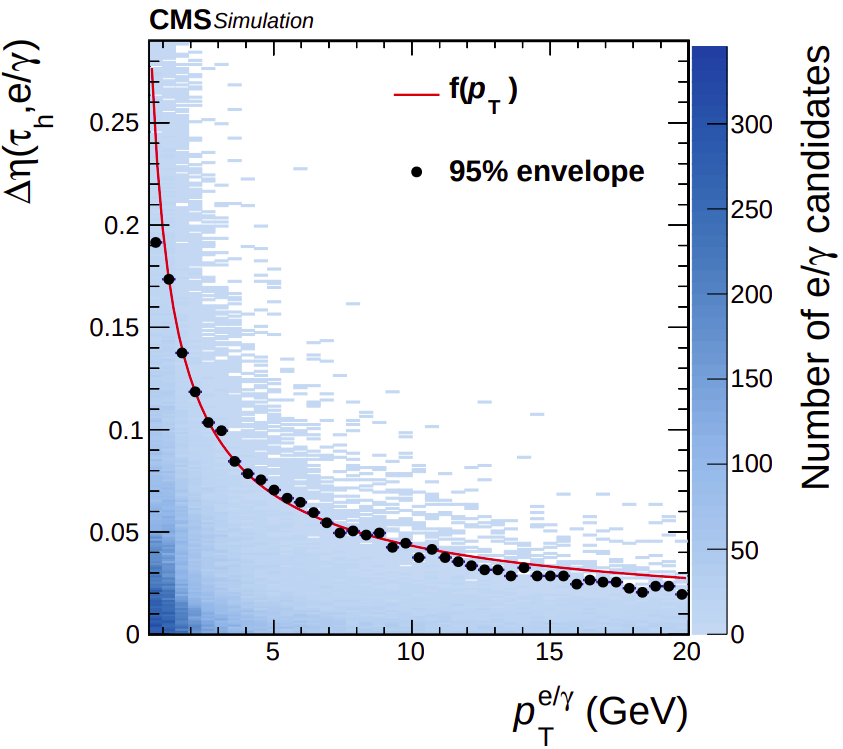
\includegraphics[width=0.5\textwidth]{Figures/hps_f.png}}
    \subfloat[]{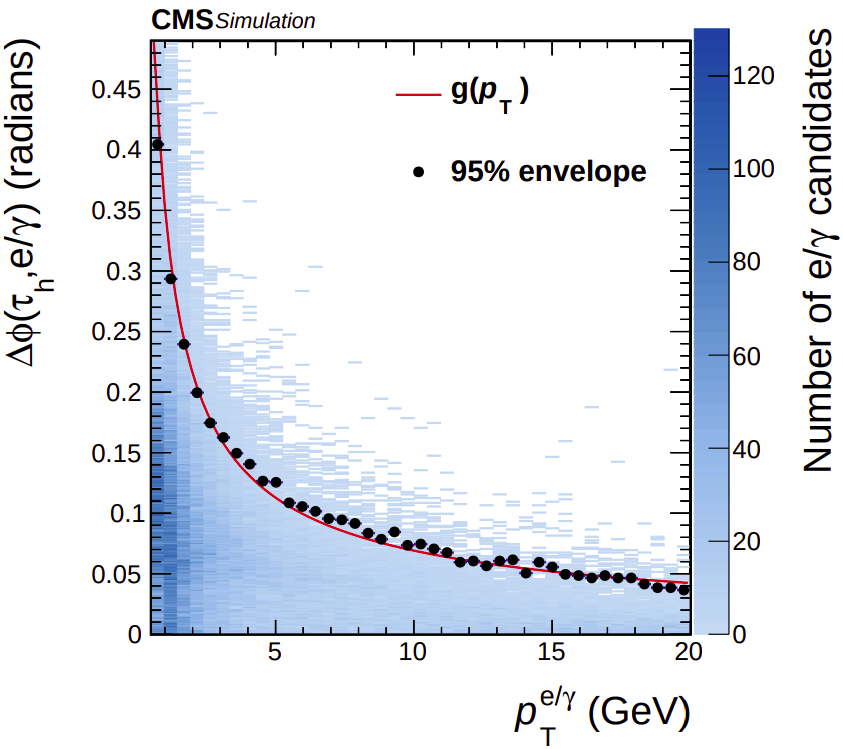
\includegraphics[width=0.5\textwidth]{Figures/hps_g.png}} \\
\caption{The distance between the hadronic tau and electron or photon $\eta$ (a) and $\phi$ (b) with respect the the electron or photon $\pT$. The binned values (points) and the fitted functions $f$ and $g$ (red line), that encapsulates 95\% of all electron and photons are shown in both cases~\cite{Sirunyan:2018pgf}.}
\label{fig:hps}
\end{figure}

Charged hadrons (prongs) are also required to have $\pT > 0.5$ GeV and originate from the \ac{PV}, with a loose transverse impact parameter of $d_{xy} < 0.1$ cm
Further constraints are placed on the reconstructed masses of the specific resonances produced by a hadronic tau decay, if produced by the decay.
In particular, the visible mass positions and widths of the grouped charged hadrons and strips are optimised to match the $\rho$ (770 MeV) and $a_1$ (1260 MeV) decays.
This is performed to maximise the fraction of hadronic tau efficiency to the probability of misidentification from jets.
The visible decay products of each decay shown in Tab~\ref{tab:tau_decay} are reconstructed by:

\begin{enumerate}[i)]
\item $h^- \pi^0$: One charged hadron candidate and no strips.
\item $h^-$: One charged hadron candidate and one strip with mass $ 0.3 < m_{\tau} < 1.3 \sqrt{p_{\text{T}}/100}$ GeV. The mass is required to be between 1.3 and 4.2 GeV.
\item $\pi^- \pi^- \pi^+$: Three charged hadron candidates with mass $0.8 < m_{\tau} < 1.5$ GeV. The tracks are required to originate within $\Delta z<0.4$ cm of the same vertex.
\item $h^- 2\pi^0$: One charged hadron candidate and two strips. The $\tau_{h}$ mass should be $0.4 < m_{\tau} < 1.2\sqrt{p_{\text{T}}/100}$~GeV. The mass is required to be between 1.2 and 4.0 GeV.
\item $\pi^- \pi^- \pi^+ \pi^0$: Three charged hadron candidates and one strip.
\end{enumerate}

The remaining hadronic decays of the tau leptons are not included in this thesis.
The \ac{DM} of the hadronic tau that is reconstructed by a \ac{HPS} is quantified by the following formula relating the number of charged hadron candidates $N_C$ and the number of strips $N_N$.

\begin{equation}
\text{DM} = 5(N_{C} - 1) + N_{N}
\end{equation}

The second step of the identification, comes from a multiclass \ac{DNN}-based algorithm named \texttt{DeepTau}, that seeks to discriminate hadronic tau decays from electron, muons, and most importantly quark or gluon jets, that can be misidentified as hadronic tau decays~\cite{CMS:2022prd}.
It uses a \ac{DNN} architecture that consists of multiple interconnected layers of nodes, that attempts to learn whether the input object is an hadronic tau decay, an electron, a muon or a jet. 
The algorithm takes inputs from reconstructed particles surrounding the \ac{HPS} hadronic tau candidate, including information about energies, momenta, and spatial positions. 
Convolutional layers are used to efficiently process these inputs by dividing them into smaller regions in $\eta$-$\phi$ space, which allows the algorithm to extract local patterns and features. 
It also incorporates high-level features of the hadronic tau candidate calculated from the \ac{HPS} algorithm, such as the four-momentum, charge, \ac{DM}, isolation variables used in previous \ac{MVA}~\cite{CMS:2018jrd}, impact parameters, $\eta$ and $\phi$ strip information, as well as event level information such as variables related to the $\ac{PU}$.
The architecture of algorithm is shown in Figure~\ref{fig:deeptau}. \\

\begin{figure}[!hbtp]
\centering
    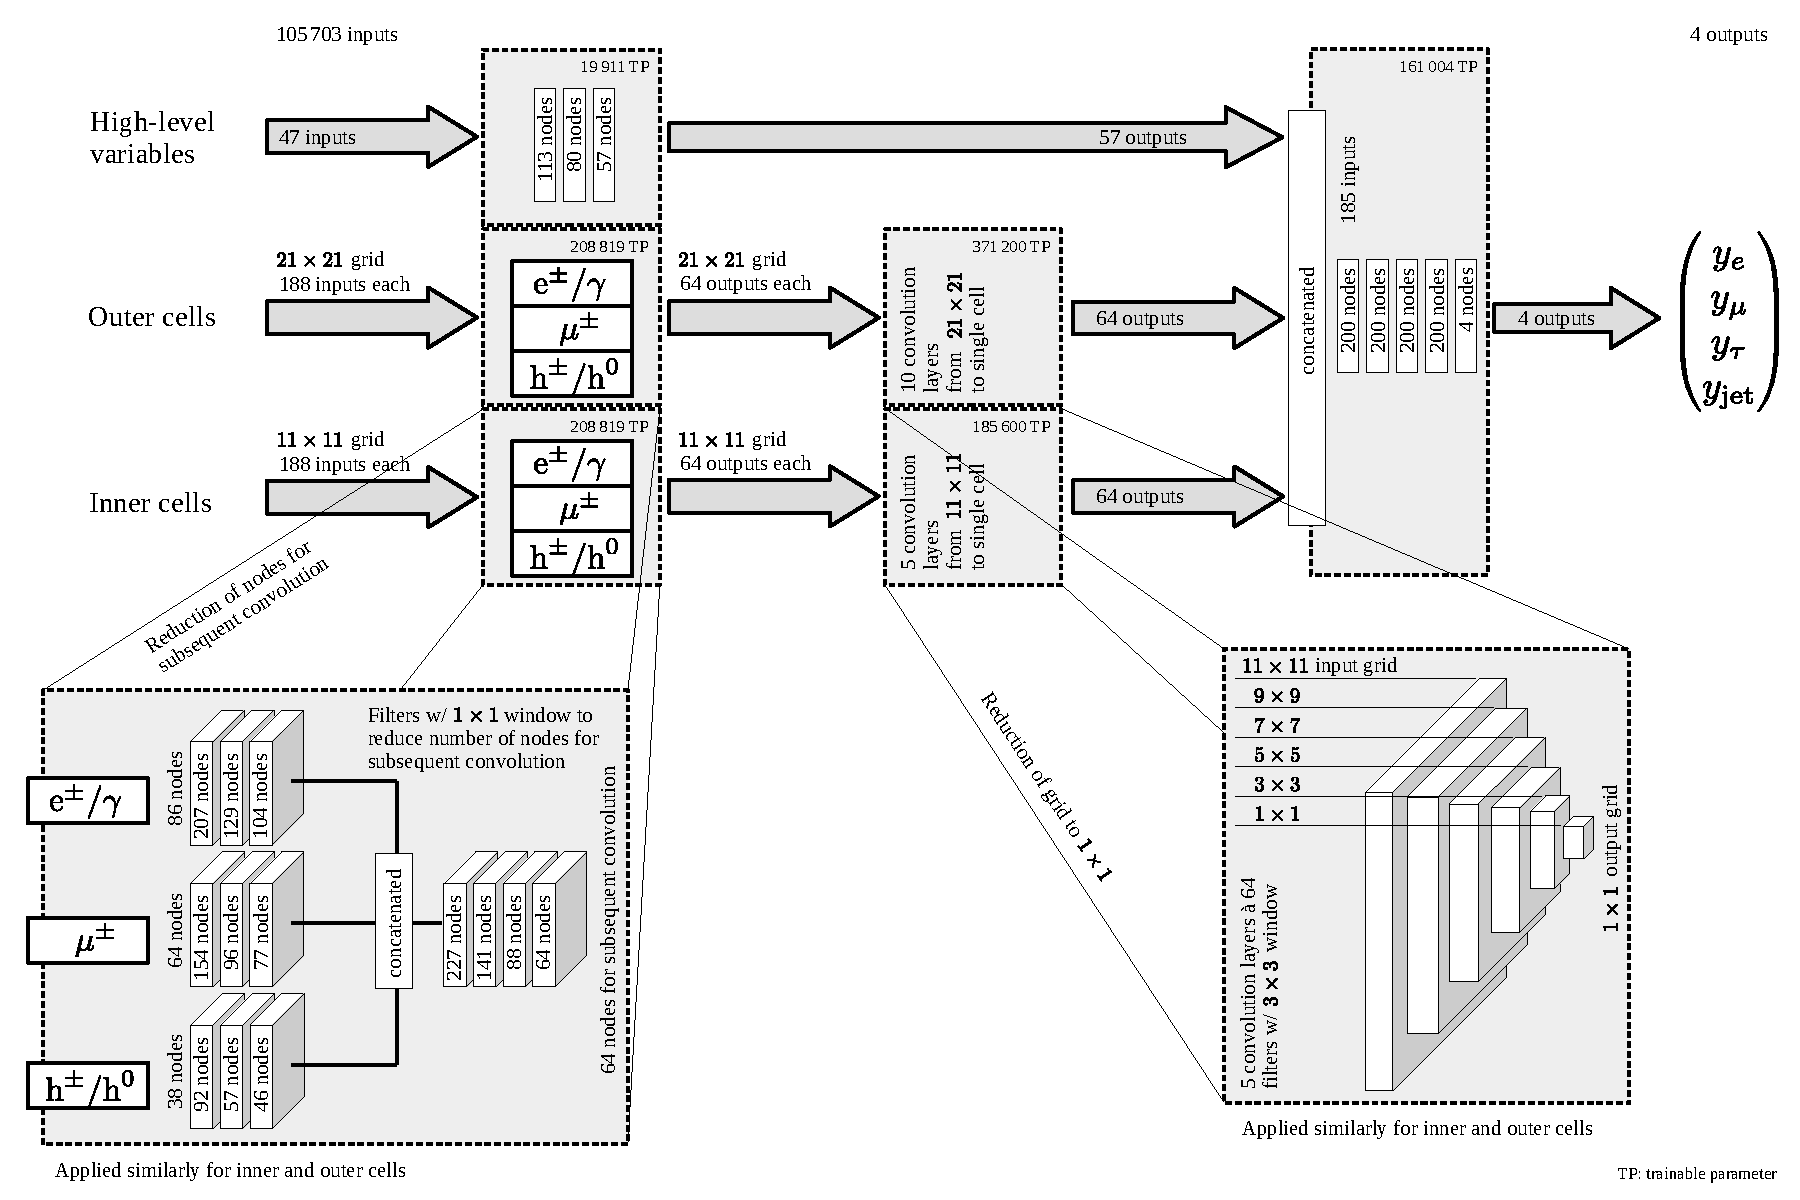
\includegraphics[width=\textwidth]{Figures/deeptau.pdf}
\caption{The architecture of the \texttt{DeepTau} neural network, comprising of three sets of input variables: inner cells, outer cells, and high-level features. These sets are processed separately through subnetworks and their outputs are concatenated. Five fully connected layers process the concatenated output to calculate the probabilities for a candidate to be a hadronic tau, electron, muon, or jet. The high-level input subnetwork consists of three fully connected layers, taking 47 inputs and yielding 57 outputs. Complex subnetworks process the features of inner and outer cells separately, with fully connected layers followed by concatenation and additional fully connected layers. Convolutional layers progressively reduce the grid size for both inner and outer cells. For inner cells, there are 5 convolutional layers, while for outer cells, there are 10 convolutional layers. The number of trainable parameters (TP) for the different subnetworks are also provided~\cite{CMS:2022prd}.}
\label{fig:deeptau}
\end{figure}

The \texttt{DeepTau} \ac{DNN} is trained using a large dataset, incorporating examples of hadronic tau decays and background processes of electrons, muons and jets. 
The output of the \ac{DNN} is 4 scores, that represent the probability that the object is a hadronic tau ($y_\tau$), an electon ($y_e$), a muon ($y_\mu$) or a jet ($y_{\text{jet}}$).
From these raw scores, additional scores are calculated for the probability that an object is a hadronic tau rather than an electron, muon or jet.
These are defined as,

\begin{equation}
D_{i}^{\text{score}} = \frac{y_\tau}{y_i + y_{\tau}}, \hspace{1cm} i \in (e,\mu,\text{jet}).
\end{equation}

From this, \ac{WP}s are defined to match specific efficiencies of hadronic tau identification with respect to each of the other 3 objects, named $D_{e}^{\text{WP}}$, $D_{\mu}^{\text{WP}}$ and $D_{\text{jet}}^{\text{WP}}$.
The target efficiencies for different \ac{WP} are shown in Table~\ref{tab:deeptau_eff}. \\

\begin{table}[!hbtp]
\begin{adjustwidth}{-1cm}{-1cm}
\centering
\begin{tabular}{|c|cccccccc|}
\hline
WP                     & VVTight & VTight & Tight  & Medium & Loose  & VLoose  & VVLoose & VVVLoose \\
\hline 
\hline
$D_{e}^{\text{WP}}$    & 60\%    & 70\%   & 80\%   & 90\%   & 95\%   & 98\%    & 99\%    & 99.5\%   \\
$D_{\mu}^{\text{WP}}$  & -       & -      & 99.5\% & 99.8\% & 99.9\% & 99.95\% & -       & -        \\
$D_{\tau}^{\text{WP}}$ & 40\%    & 50\%   & 60\%   & 70\%   & 80\%   & 90\%    & 95\%    & 98\%     \\
\hline
\end{tabular}
\caption{Target efficiencies of the \texttt{DeepTau} working points with respect to electrons, muons and jets.}
\label{tab:deeptau_eff}
\end{adjustwidth}
\end{table}

Due to the lack of muons misidentified as hadronic taus, high efficiencies can be required for $D_{\mu}^{\text{WP}}$.
This is also the reason for why the target efficiencies for $D_{e}^{\text{WP}}$ are higher than for $D_{\text{jet}}^{\text{WP}}$, where the large challenge jets misidentified as hadronic taus is present.
The misidentification probabilities for the different hadronic tau efficiencies are shown in Figure~\ref{fig:deeptau_misid}.
Also shown in these plots, is the performance comparison to an older \ac{MVA} algorithm for electrons and jets, as well as a cut based algorithm for muons, both described in Reference~\cite{CMS:2018jrd}.
Significant improvements with respect to the previous algorithm is observed, which has a results in a significant improvement in analyses utilising tau leptons at the CMS experiment.
The different $D_{e}^{\text{WP}}$, $D_{\mu}^{\text{WP}}$ and $D_{\text{jet}}^{\text{WP}}$ can be used to optimise the hadronic tau identification for analyses attempting to separate tau enriched signals from backgrounds of misidentified objects.
Two examples of analyses that utilise this are described in Chapter~\ref{sec:bsm_H_to_tau_tau_analysis} and \ref{sec:H_A_to_4_tau_analysis}.

\begin{figure}[!hbtp]
\centering
    \subfloat[]{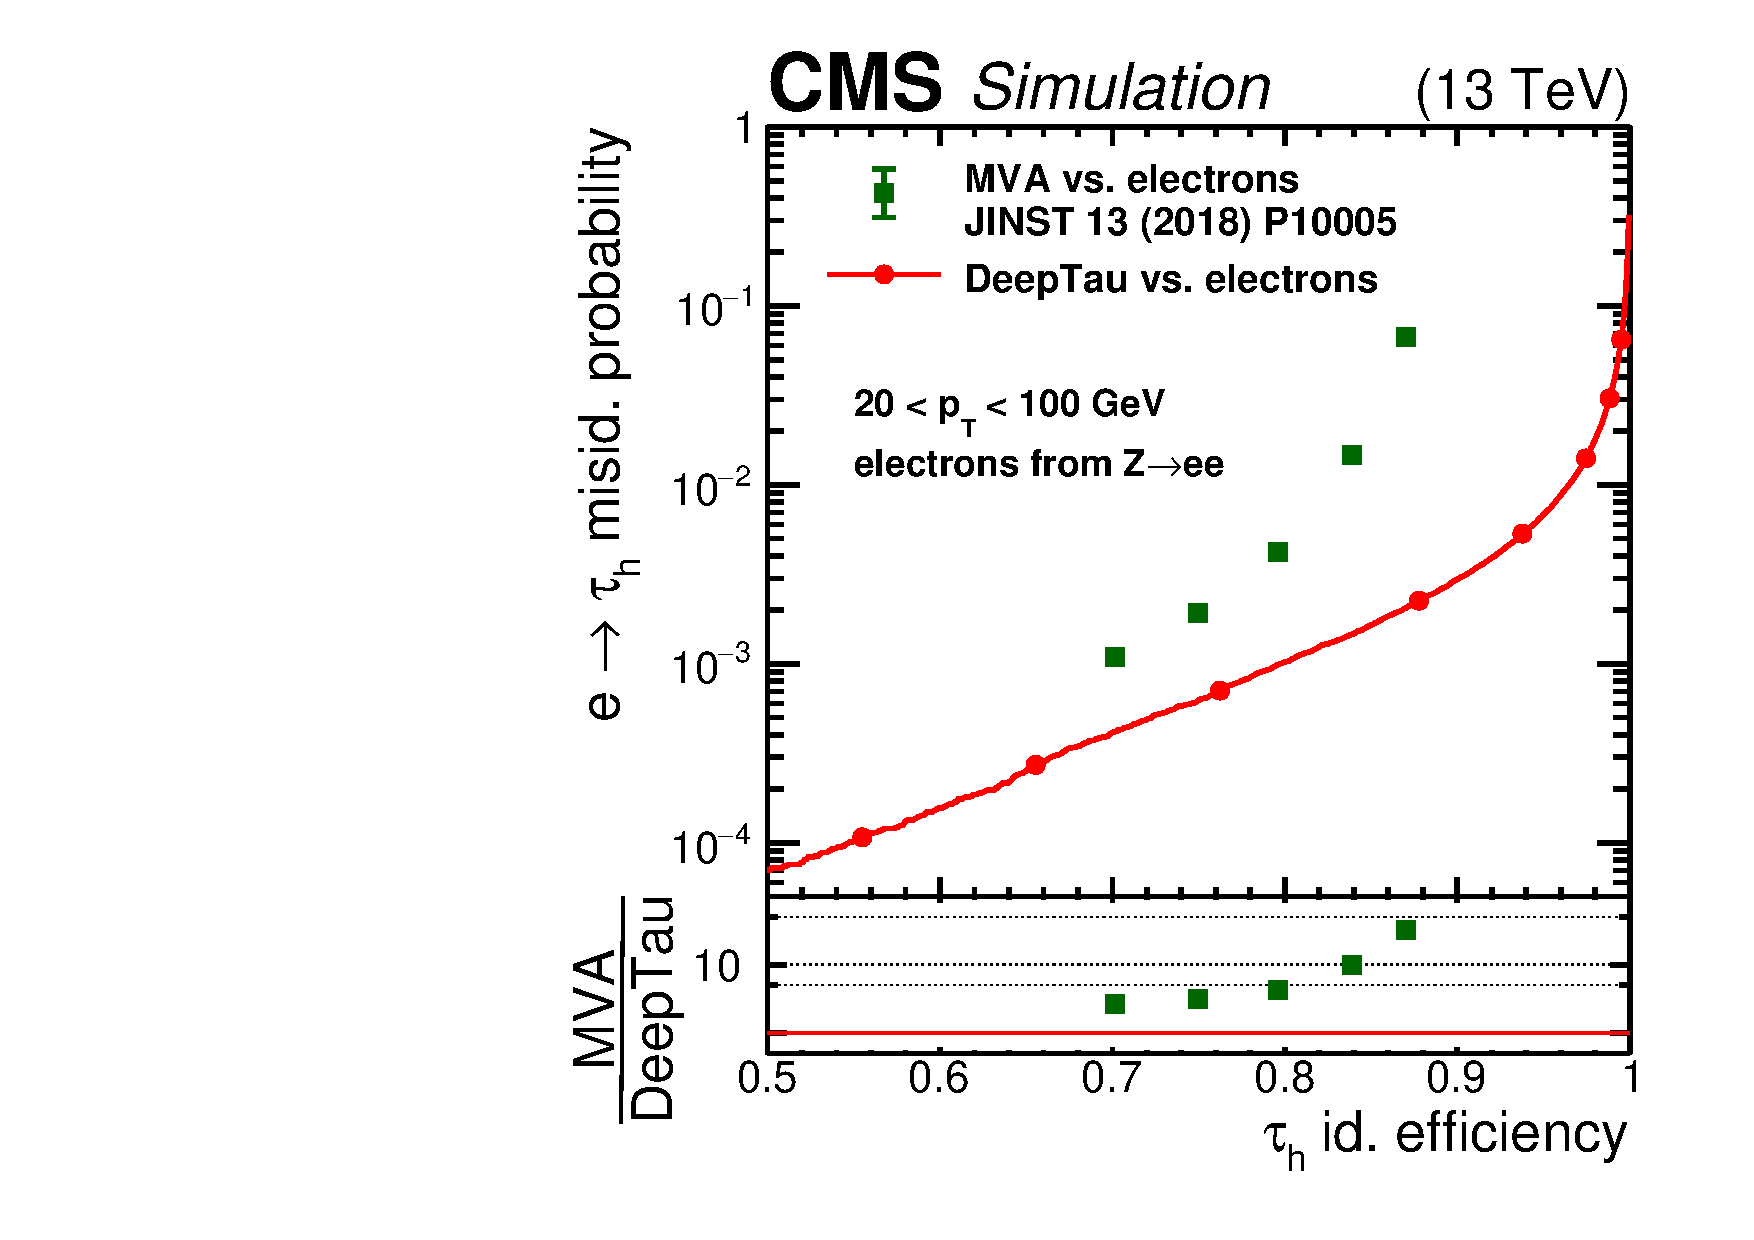
\includegraphics[width=0.5\textwidth]{Figures/deeptau_misid_electron.pdf}}
    \subfloat[]{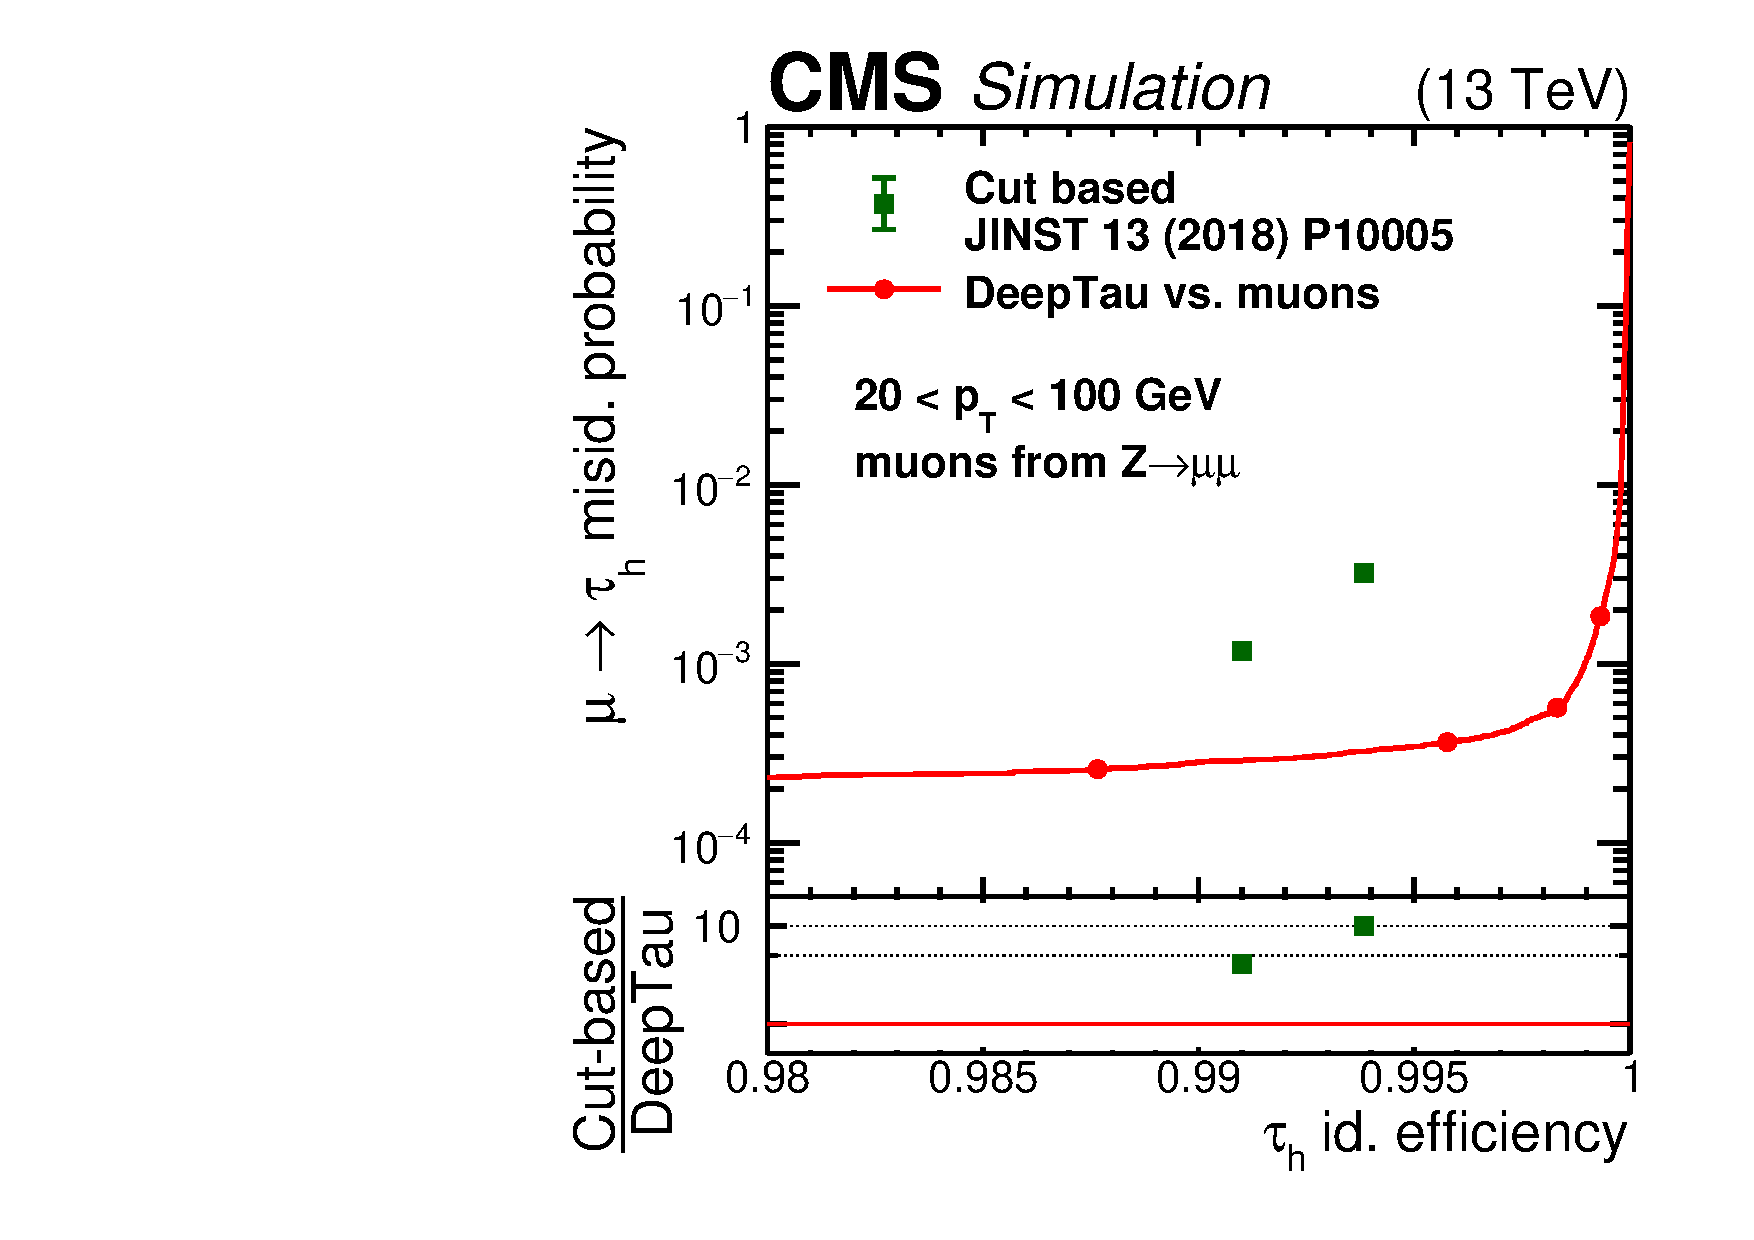
\includegraphics[width=0.5\textwidth]{Figures/deeptau_misid_muon.pdf}} \\
    \subfloat[]{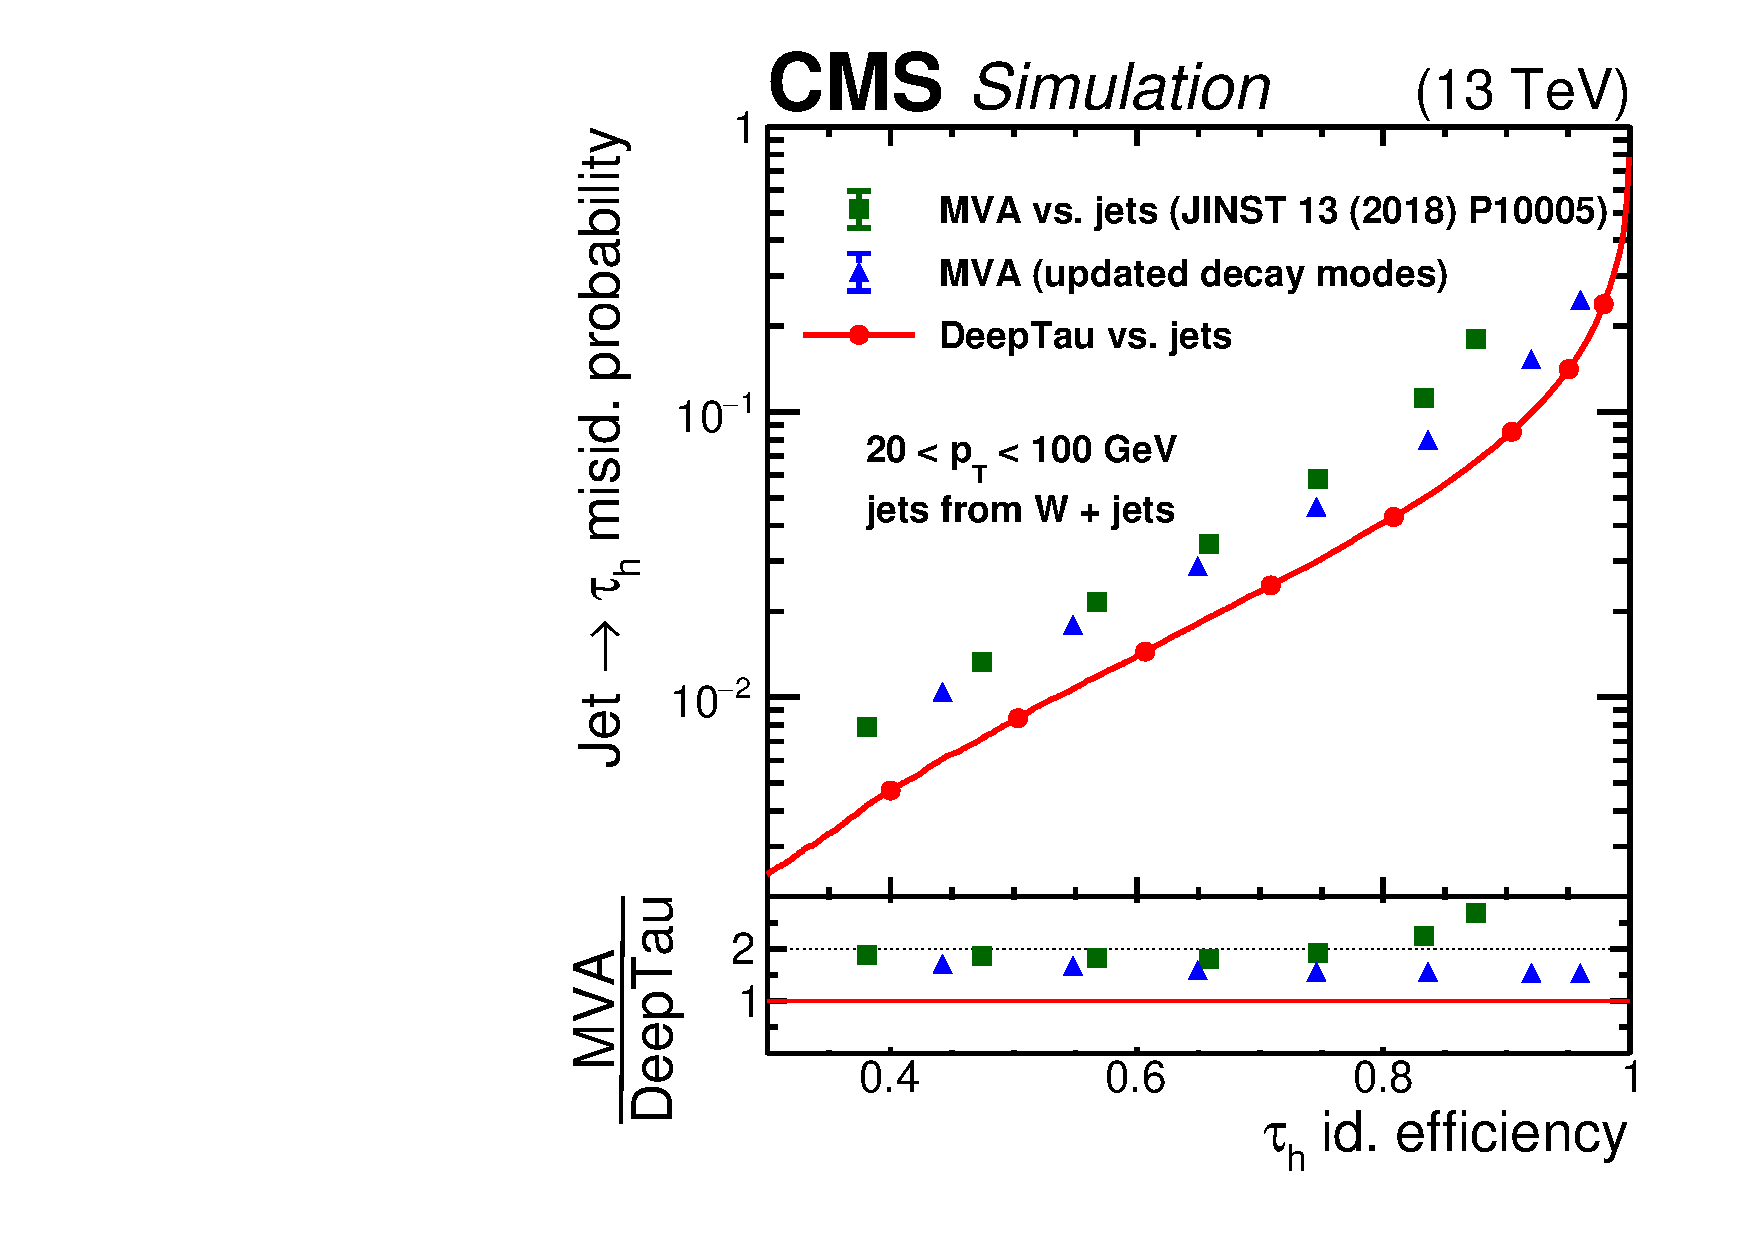
\includegraphics[width=0.5\textwidth]{Figures/deeptau_misid_jet.pdf}}
\caption{Efficiency comparisons of electrons (a), muons (b) and jets (c) passing the \texttt{DeepTau} identification discriminators versus hadronic tau efficiency. (a) uses $Z\rightarrow ee$, (b) uses $Z\rightarrow \mu\mu$ and (c) uses W+jets MC, with only objects with $\pT<100$ GeV used. Working points are indicated by full circles and previous algorithms described in Reference~\cite{CMS:2018jrd} are shown in blue triangles and green squares~\cite{CMS:2022prd}.}
\label{fig:deeptau_misid}
\end{figure}